 
\documentclass{beamer}

\usepackage[utf8]{inputenc}
\usepackage[spanish]{babel}
\usepackage[T1]{fontenc}
\usepackage{color}

\title{La comercializacion actual de productos alimenticios y bebidas en el municipio  Centro Habana.}

\includegraphics[scale=0.6]{matcom.png}
\author{Vicente Cao Tarrero\\Facultad Matematica y Computación}
\usetheme{Berlin}
\begin{document}

\begin{frame}
\titlepage{}
\end{frame}

\newpage

\begin{frame}
\tableofcontents
\end{frame}

\section{Introducción}
\begin{frame}
\frametitle{Introducción}

La difícil situación económica de Cuba impacta los precios de productos como la cerveza, cebolla y calabaza en el mercado informal de Centro Habana. En especial, la cerveza que es un producto mayormente importado al pais y se comercializa al por mayor en los almacenes estatales.

\end{frame}

\section{Info. Centro Habana}
\begin{frame}
\frametitle{Información Centro Habana}

Centro Habana tiene una extensión de 3.42 km2 lo cual representa el 0.47 porciento de todo el territorio capitalino y una población densa. Es un territorio totalmente urbanizado que posee 514 manzanas sin espacios libres. Está rodeado por el litoral norte, La Habana Vieja al este, el Cerro al sur y Playa al oeste.

\end{frame}

\section{Objetivo}
\begin{frame}
\frametitle{Objetivo}

Explorar efectos de la comercialización de cerveza, cebolla y calabaza en el municipio.

\end{frame}

\newpage
\section{Análisis}
\begin{frame}
\frametitle{Análisis}\\Cerveza mas vendida
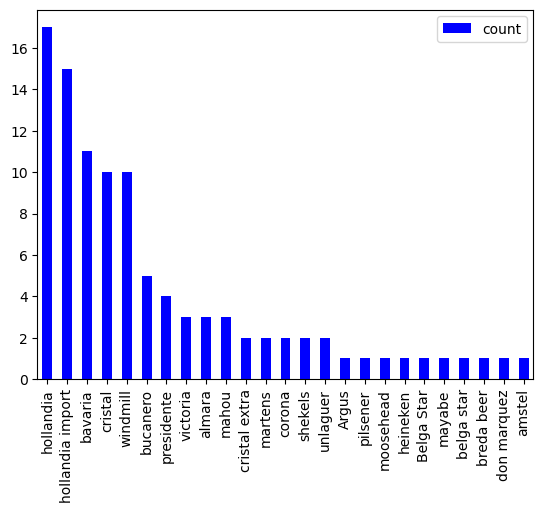
\includegraphics[width=0.7\textwidth]{Cerv_mas_vendida.png}
\end{frame}

\newpage
\begin{frame}
\frametitle{Análisis}\\Tipo de envace
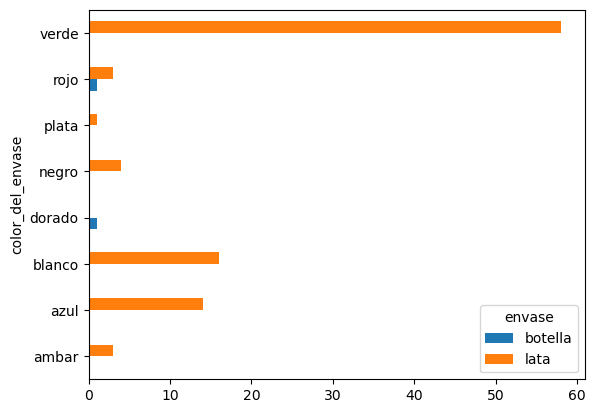
\includegraphics[width=0.8\textwidth]{Cerv_tipo_de_envace.png}
\end{frame}

\newpage
\begin{frame}
\frametitle{Análisis}\\Contenido en ml contra precio
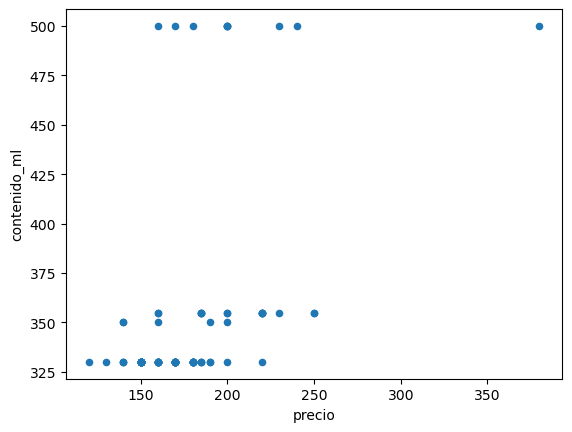
\includegraphics[width=0.7\textwidth]{Cerv_tipo_de_envace_precio.png}
\end{frame}

\newpage
\begin{frame}
\frametitle{Análisis}
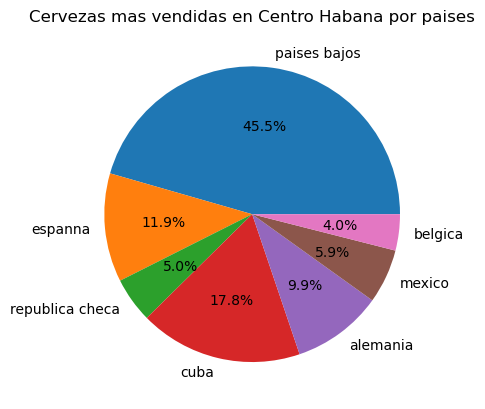
\includegraphics[width=0.7\textwidth]{Cerv_mas_vendida_por_pais.png}
\end{frame}

\newpage
\begin{frame}
\frametitle{Análisis}
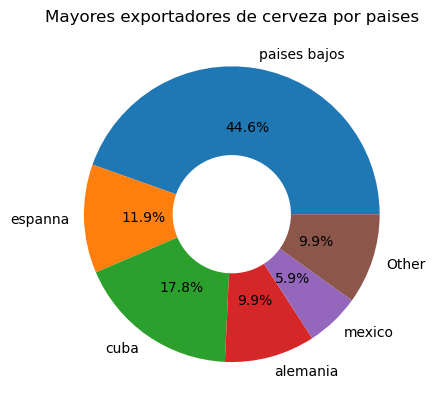
\includegraphics[width=0.7\textwidth]{Cerv_mayor_exportador.png}
\end{frame}

\newpage
\begin{frame}
\frametitle{Análisis}\\Tipos de ventas de Cebolla
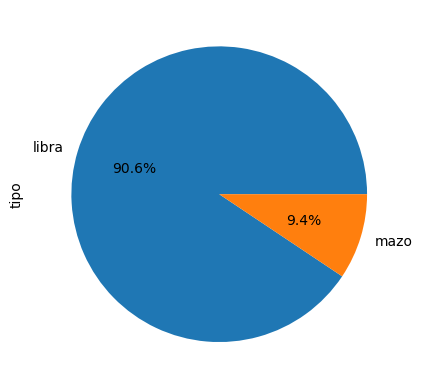
\includegraphics[width=0.7\textwidth]{Ceb_tipos_de_ventas.png}
\end{frame}

\newpage
\begin{frame}
\frametitle{Análisis}\\Cebolla mas vendida
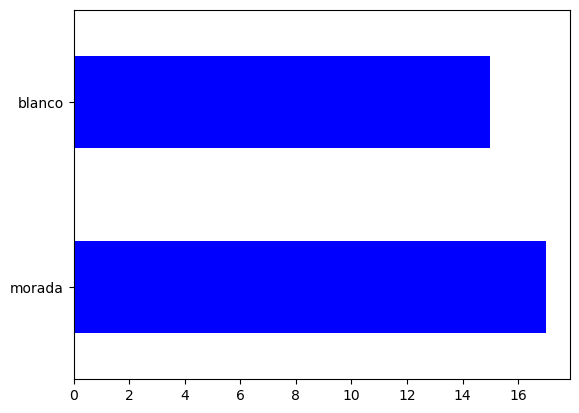
\includegraphics[width=0.7\textwidth]{Ceb_mas_vendida.png}
\end{frame}

\newpage
\begin{frame}
\frametitle{Análisis}
La calabaza se expende por libras y tiene un precio equivalente en los difentes segmentos del mercado, que oscila entre 40 y 60 pesos la libra.
\end{frame}


\section{Conclusiones}
\begin{frame}
\frametitle{Conclusiones}

La comercialización de estos productos podría optimizarse en beneficio de vendedores y consumidores. Se requiere continuar análisis de evolución de precios y hábitos de consumo segun la oferta realizada.S

\end{frame}

\end{document}